\documentclass{standalone}
\usepackage{tikz}
\usetikzlibrary{patterns, positioning}

\begin{document}
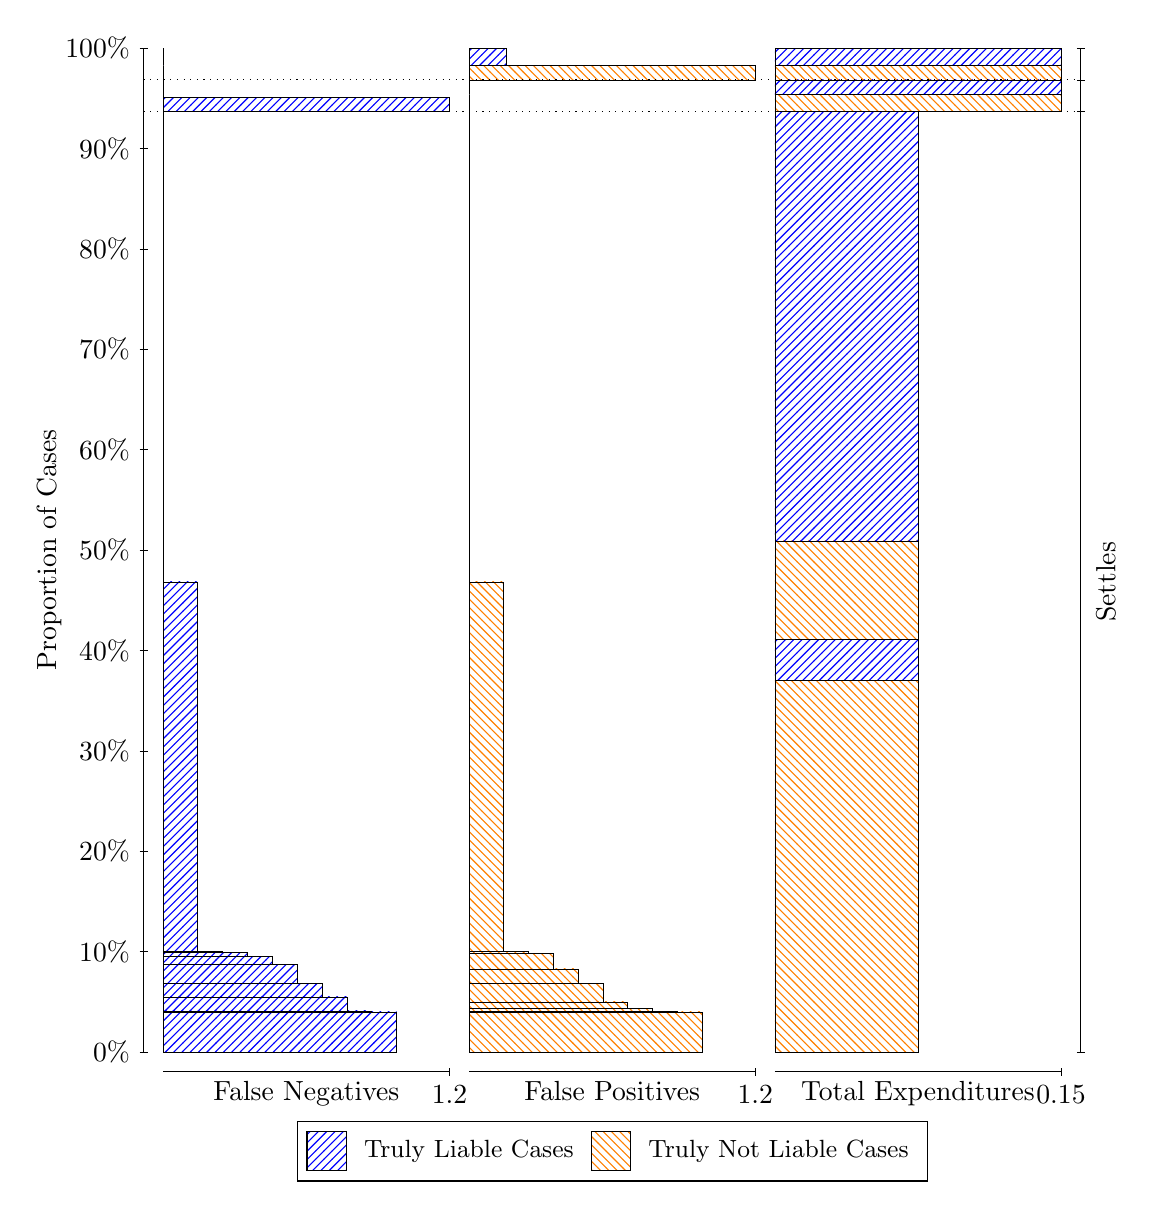
\begin{tikzpicture}
\draw[black, very thin] (1.5,1.75) -- (1.5,14.5);
\node[rotate=90, anchor=center] at (0.3, 8.125) {Proportion of Cases};
\draw[black, very thin] (1.45,1.75) -- (1.55,1.75);
\node[anchor=east] at (1.45, 1.75) {0\%};
\draw[black, very thin] (1.45,3.025) -- (1.55,3.025);
\node[anchor=east] at (1.45, 3.025) {10\%};
\draw[black, very thin] (1.45,4.3) -- (1.55,4.3);
\node[anchor=east] at (1.45, 4.3) {20\%};
\draw[black, very thin] (1.45,5.575) -- (1.55,5.575);
\node[anchor=east] at (1.45, 5.575) {30\%};
\draw[black, very thin] (1.45,6.85) -- (1.55,6.85);
\node[anchor=east] at (1.45, 6.85) {40\%};
\draw[black, very thin] (1.45,8.125) -- (1.55,8.125);
\node[anchor=east] at (1.45, 8.125) {50\%};
\draw[black, very thin] (1.45,9.4) -- (1.55,9.4);
\node[anchor=east] at (1.45, 9.4) {60\%};
\draw[black, very thin] (1.45,10.675) -- (1.55,10.675);
\node[anchor=east] at (1.45, 10.675) {70\%};
\draw[black, very thin] (1.45,11.95) -- (1.55,11.95);
\node[anchor=east] at (1.45, 11.95) {80\%};
\draw[black, very thin] (1.45,13.225) -- (1.55,13.225);
\node[anchor=east] at (1.45, 13.225) {90\%};
\draw[black, very thin] (1.45,14.5) -- (1.55,14.5);
\node[anchor=east] at (1.45, 14.5) {100\%};

\draw[black, very thin] (13.4,1.75) -- (13.4,14.5);
\draw[black, very thin] (13.35,1.75) -- (13.45,1.75);
\node[anchor=west] at (13.35, 1.75) {};
\draw[black, very thin] (13.35,13.691) -- (13.45,13.691);
\node[anchor=west] at (13.35, 13.691) {};
\draw[black, very thin] (13.35,14.095) -- (13.45,14.095);
\node[anchor=west] at (13.35, 14.095) {};
\draw[black, very thin] (13.35,14.5) -- (13.45,14.5);
\node[anchor=west] at (13.35, 14.5) {};

\draw[black, very thin, pattern color=blue, pattern=north east lines] (1.75,1.75) rectangle (4.712,2.2583);
\draw[black, very thin, pattern color=blue, pattern=north east lines] (1.75,2.2583) rectangle (4.396,2.2717);
\draw[black, very thin, pattern color=blue, pattern=north east lines] (1.75,2.2717) rectangle (4.0801,2.4508);
\draw[black, very thin, pattern color=blue, pattern=north east lines] (1.75,2.4508) rectangle (3.7641,2.6254);
\draw[black, very thin, pattern color=blue, pattern=north east lines] (1.75,2.6254) rectangle (3.4482,2.8655);
\draw[black, very thin, pattern color=blue, pattern=north east lines] (1.75,2.8655) rectangle (3.1322,2.9616);
\draw[black, very thin, pattern color=blue, pattern=north east lines] (1.75,2.9616) rectangle (2.8163,3.0171);
\draw[black, very thin, pattern color=blue, pattern=north east lines] (1.75,3.0171) rectangle (2.5004,3.0284);
\draw[black, very thin, pattern color=blue, pattern=north east lines] (1.75,3.0284) rectangle (2.1844,7.7202);
\draw[black, very thin, pattern color=orange, pattern=north west lines] (1.75,7.7202) rectangle (1.75,13.691);
\draw[black, very thin, pattern color=blue, pattern=north east lines] (1.75,13.691) rectangle (5.3833,13.875);
\draw[black, very thin, pattern color=orange, pattern=north west lines] (1.75,13.875) rectangle (1.75,14.095);
\draw[black, very thin, pattern color=orange, pattern=north west lines] (1.75,14.095) rectangle (1.75,14.28);
\draw[black, very thin, pattern color=blue, pattern=north east lines] (1.75,14.28) rectangle (1.75,14.5);
\draw[black, very thin, pattern color=orange, pattern=north west lines] (5.6333,1.75) rectangle (8.5953,2.2583);
\draw[black, very thin, pattern color=orange, pattern=north west lines] (5.6333,2.2583) rectangle (8.2793,2.2637);
\draw[black, very thin, pattern color=orange, pattern=north west lines] (5.6333,2.2637) rectangle (7.9634,2.3042);
\draw[black, very thin, pattern color=orange, pattern=north west lines] (5.6333,2.3042) rectangle (7.6475,2.3856);
\draw[black, very thin, pattern color=orange, pattern=north west lines] (5.6333,2.3856) rectangle (7.3315,2.6257);
\draw[black, very thin, pattern color=orange, pattern=north west lines] (5.6333,2.6257) rectangle (7.0156,2.7949);
\draw[black, very thin, pattern color=orange, pattern=north west lines] (5.6333,2.7949) rectangle (7.0156,2.8062);
\draw[black, very thin, pattern color=orange, pattern=north west lines] (5.6333,2.8062) rectangle (6.6996,3.0004);
\draw[black, very thin, pattern color=orange, pattern=north west lines] (5.6333,3.0004) rectangle (6.3837,3.0284);
\draw[black, very thin, pattern color=orange, pattern=north west lines] (5.6333,3.0284) rectangle (6.0678,7.7203);
\draw[black, very thin, pattern color=blue, pattern=north east lines] (5.6333,7.7203) rectangle (5.6333,13.691);
\draw[black, very thin, pattern color=orange, pattern=north west lines] (5.6333,13.691) rectangle (5.6333,13.911);
\draw[black, very thin, pattern color=blue, pattern=north east lines] (5.6333,13.911) rectangle (5.6333,14.095);
\draw[black, very thin, pattern color=orange, pattern=north west lines] (5.6333,14.095) rectangle (9.2667,14.28);
\draw[black, very thin, pattern color=blue, pattern=north east lines] (5.6333,14.28) rectangle (6.1072,14.5);
\draw[black, very thin, pattern color=orange, pattern=north west lines] (9.5167,1.75) rectangle (11.333,6.4699);
\draw[black, very thin, pattern color=blue, pattern=north east lines] (9.5167,6.4699) rectangle (11.333,6.9916);
\draw[black, very thin, pattern color=orange, pattern=north west lines] (9.5167,6.9916) rectangle (11.333,8.2419);
\draw[black, very thin, pattern color=blue, pattern=north east lines] (9.5167,8.2419) rectangle (11.333,13.691);
\draw[black, very thin, pattern color=orange, pattern=north west lines] (9.5167,13.691) rectangle (13.15,13.911);
\draw[black, very thin, pattern color=blue, pattern=north east lines] (9.5167,13.911) rectangle (13.15,14.095);
\draw[black, very thin, pattern color=orange, pattern=north west lines] (9.5167,14.095) rectangle (13.15,14.28);
\draw[black, very thin, pattern color=blue, pattern=north east lines] (9.5167,14.28) rectangle (13.15,14.5);
\draw[black, dotted] (1.5,13.691) -- (13.4,13.691);
\draw[black, dotted] (1.5,14.095) -- (13.4,14.095);
\draw[black, very thin] (1.75,1.5) -- (5.3833,1.5);
\node[anchor=north] at (3.5667, 1.5) {False Negatives};
\draw[black, very thin] (5.3833,1.45) -- (5.3833,1.55);
\node[anchor=north] at (5.3833, 1.45) {1.2};

\draw[black, very thin] (5.6333,1.5) -- (9.2667,1.5);
\node[anchor=north] at (7.45, 1.5) {False Positives};
\draw[black, very thin] (9.2667,1.45) -- (9.2667,1.55);
\node[anchor=north] at (9.2667, 1.45) {1.2};

\draw[black, very thin] (9.5167,1.5) -- (13.15,1.5);
\node[anchor=north] at (11.333, 1.5) {Total Expenditures};
\draw[black, very thin] (13.15,1.45) -- (13.15,1.55);
\node[anchor=north] at (13.15, 1.45) {0.15};

\node[black, centered, rotate=90] at (13.72, 7.7203) {Settles};



\draw (7.449999999999999,1.5) node[draw=none] (baseCoordinate) {};
\begin{scope}[align=center]
        \matrix[scale=0.5, draw=black, below=0.5cm of baseCoordinate, nodes={draw}, column sep=0.1cm]{
            \node[rectangle, draw, minimum width=0.5cm, minimum height=0.5cm, pattern=north east lines, pattern color=blue] {}; &
            \node[draw=none, font=\small] (B) {Truly Liable Cases}; &
            \node[rectangle, draw, minimum width=0.5cm, minimum height=0.5cm, pattern=north west lines, pattern color=orange] {}; &
            \node[draw=none, font=\small] (B) {Truly Not Liable Cases}; \\
            };
\end{scope}

\end{tikzpicture}
\end{document}